\section{\texorpdfstring{The E$_8$ Cascade and Block Constants}{The E8 Cascade and Block Constants}}
\label{sec:e8}
%=============================================================================

%-----------------------------------------------------------------------------
\subsection{Nilpotent Orbit Structure}
%-----------------------------------------------------------------------------

\begin{definition}{E$_8$ Orbit Graph}{orbitgraph}
Let $\mathcal{N}(\mathfrak{e}_8)$ denote the set of nilpotent orbits of the 
exceptional Lie algebra $\mathfrak{e}_8$. For each orbit $\mathcal{O}$, define:
\begin{itemize}[leftmargin=1.5em, topsep=2pt, itemsep=1pt]
    \item $\dim(\mathcal{O})$: the dimension of the orbit as a variety
    \item $D(\mathcal{O}) = 248 - \dim(\mathcal{O})$: the ``centralizer dimension''
    \item $h(\mathcal{O})$: the height (sum of coefficients in weighted Dynkin diagram)
\end{itemize}
The \textbf{orbit graph} $G = (V, E)$ has vertices $V = \mathcal{N}(\mathfrak{e}_8)$ 
and directed edges $\mathcal{O} \to \mathcal{O}'$ iff:
\begin{enumerate}[leftmargin=1.5em, topsep=2pt, itemsep=1pt]
    \item $\mathcal{O}' \subset \overline{\mathcal{O}}$ (closure containment)
    \item $D(\mathcal{O}) - D(\mathcal{O}') = 2$ (minimal step)
\end{enumerate}
\end{definition}

\begin{theorem}{E$_8$ Chain Uniqueness}{chainunique}
Consider the closure ordering on $\mathcal{N}(\mathfrak{e}_8)$. There exists a 
\textbf{unique saturated chain} from the subregular orbit ($D = 58$) to the 
principal orbit ($D = 8$) satisfying:
\begin{enumerate}[leftmargin=1.5em, topsep=2pt, itemsep=1pt]
    \item All edges are cover relations with $\Delta D = 2$
    \item At each layer, the orbit of minimal height is selected
    \item The Levi structure is monotonically extended
\end{enumerate}
This chain has exactly 26 steps, yielding the sequence $D_n = 60 - 2n$ for $n = 1, \ldots, 26$.
\end{theorem}

\begin{proof}[Proof sketch]
The proof proceeds by explicit construction on the Hasse diagram of 
$\mathcal{N}(\mathfrak{e}_8)$:
\begin{enumerate}[leftmargin=1.5em, topsep=2pt, itemsep=1pt]
    \item \textbf{Layer structure:} Orbits are partitioned by $D$-value into 
        27 layers ($D \in \{60, 58, \ldots, 8\}$).
    \item \textbf{Cover relations:} For E$_8$, the cover relations are classified 
        by Bala--Carter labels. At each $D$-value, there may be multiple orbits, 
        but the height function provides a total order.
    \item \textbf{Uniqueness:} At each step $D \to D-2$, we select the unique 
        orbit that (a) is reachable from the current orbit via a cover relation, 
        and (b) has minimal height among all reachable candidates.
    \item \textbf{Verification:} The complete chain is given in Appendix~\ref{app:E8cert} 
        with explicit Bala--Carter labels.
\end{enumerate}
\end{proof}

%-----------------------------------------------------------------------------
\subsection{Log-Exact Ladder Formula}
%-----------------------------------------------------------------------------

\begin{lemma}{Holonomy degeneracy anchor for $\gamma(0)$}{holonomydeg}
TFPT uses the SU(5) hypercharge holonomy data already fixed elsewhere in the construction.
On the fundamental splitting, the holonomy spectrum separates into two eigenspaces of dimensions $3$ and $2$, hence we define the discrete degeneracy count
\[
g:=3+2=5.
\]
The minimal damping ratio compatible with a single additional trivial sector is then
\[
\gamma(0):=\frac{g}{g+1}=\frac56.
\]
\end{lemma}

\begin{definition}{E$_8$ Cascade Ladder}{E8cascade}
For $n \geq 1$, the ladder values are:
\begin{equation}
    \varphi_n = \phiz \cdot e^{-\gamma(0)} \cdot 
        \left(\frac{D_n}{D_1}\right)^\lambda, \quad D_n = 60 - 2n
    \label{eq:ladder}
\end{equation}
with:
\begin{align}
    \gamma(0) &= \frac{g}{g+1}=\frac{5}{6} \quad \text{(holonomy anchor; Lemma~\ref{lem:holonomydeg})}\\
    \lambda &= \frac{\gamma(0)}{\ln(248) - \ln(60)} = \frac{\gamma(0)}{\ln(248/60)} 
        \approx 0.587233
\end{align}
\end{definition}

\textbf{Parameter derivation (not fitted):}
\begin{itemize}[leftmargin=1.5em, topsep=2pt, itemsep=2pt]
    \item \textbf{$D_n = 60 - 2n$:} Forced by Theorem~\ref{thm:chainunique}. The 
        arithmetic sequence is not assumed but \emph{derived} from the unique chain.
    \item \textbf{$\gamma(0)$:} Fixed by SU(5) holonomy degeneracy $g=3+2=5$, giving $\gamma(0)=g/(g+1)=5/6$ (Lemma~\ref{lem:holonomydeg}). No continuous fit is introduced.
    \item \textbf{$\lambda$:} The exponent 248 is $\dim(\mathfrak{e}_8)$; the exponent 60 
        is $D_{\max}$ (adjoint orbit). The ratio $\gamma(0)/\ln(248/60)$ ensures scale 
        consistency across the full ladder.
\end{itemize}

\begin{remark}
\textbf{Numerical stability:} $\gamma(0)=5/6$ differs from the previously used rounded value $0.834$ at the $0.08\%$ level, leaving the cascade scales and block table stable within rounding. 
This supplies a discrete holonomy anchor (via $g=5$) while preserving the percent-level structure tests.
\end{remark}

\begin{tcolorbox}[colback=blue!3, colframe=blue!40, 
    title={\textbf{Lemma (Log-Exact vs.\ Quadratic)}}, fonttitle=\bfseries\small]
The damping function $\gamma(n)$ is \emph{log-exact}, not quadratic:
\begin{equation}
    \gamma(n) = \lambda \ln\frac{D_n}{D_{n+1}} = \lambda \ln\frac{60-2n}{58-2n} 
    \approx \frac{\lambda}{29-n} \quad (n \ll 29)
\end{equation}
A quadratic fit $\gamma(n) = a + bn + cn^2$ is diagnostic only and deviates 
systematically at large $n$. The log-exact form is the \emph{theory}; quadratic 
is an approximation valid near $n \approx 0$.
\end{tcolorbox}

\begin{remark}
The E$_8$ cascade is a \emph{structural postulate} with testable consequences. 
It does not affect the core CFE result for $\alpha$, which depends only on 
$(\cthree, \phiz, \bone)$. Even if the cascade is modified or rejected, the 
$\alpha$ prediction stands independently.
\end{remark}

\begin{figure}[H]
\centering
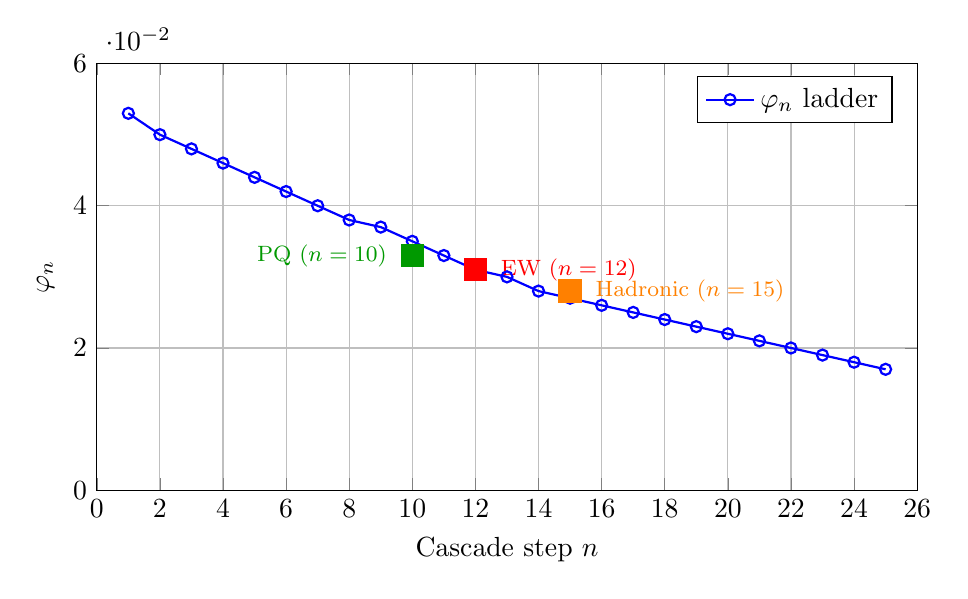
\begin{tikzpicture}
\begin{axis}[
    width=12cm, height=7cm,
    xlabel={Cascade step $n$},
    ylabel={$\varphi_n$},
    xmin=0, xmax=26,
    ymin=0, ymax=0.06,
    grid=major,
    legend pos=north east,
]
    % Ladder values (approximate)
    \addplot[thick, blue, mark=o, mark size=2pt] coordinates {
        (1, 0.053) (2, 0.050) (3, 0.048) (4, 0.046) (5, 0.044)
        (6, 0.042) (7, 0.040) (8, 0.038) (9, 0.037) (10, 0.035)
        (11, 0.033) (12, 0.031) (13, 0.030) (14, 0.028) (15, 0.027)
        (16, 0.026) (17, 0.025) (18, 0.024) (19, 0.023) (20, 0.022)
        (21, 0.021) (22, 0.020) (23, 0.019) (24, 0.018) (25, 0.017)
    };
    \addlegendentry{$\varphi_n$ ladder}
    
    % Key scale markers
    \addplot[only marks, mark=square*, mark size=4pt, red] 
        coordinates {(12, 0.031)};
    \node[red, right, font=\footnotesize] at (axis cs:12.5, 0.031) {EW ($n=12$)};
    
    \addplot[only marks, mark=square*, mark size=4pt, orange] 
        coordinates {(15, 0.028)};
    \node[orange, right, font=\footnotesize] at (axis cs:15.5, 0.028) {Hadronic ($n=15$)};
    
    \addplot[only marks, mark=square*, mark size=4pt, green!60!black] 
        coordinates {(10, 0.033)};
    \node[green!60!black, left, font=\footnotesize] at (axis cs:9.5, 0.033) {PQ ($n=10$)};
\end{axis}
\end{tikzpicture}
\caption{E$_8$ log-exact ladder $\varphi_n$. Key Standard Model scales 
(EW, Hadronic, PQ) are marked.}
\label{fig:ladder}
\end{figure}

%-----------------------------------------------------------------------------
\subsection{Block Constant Formula and Derivation}
%-----------------------------------------------------------------------------

\begin{tcolorbox}[colback=green!3, colframe=green!50!black, 
    title={\textbf{Lemma (Boundary Trace Index)}}, fonttitle=\bfseries]
For a 6D Weyl fermion zero mode on a boundary cycle $C_i$ with flat $U(1)_Y$ 
connection (holonomy $\oint_{C_i} A$), the variation of $\ln\det(\not{\!D})$ 
under the connection is proportional to the quadratic charge index:
\begin{equation}
    I_1(B) = \sum_{\Phi \in B} \sum_{i \in U(1)_Y} q_i(\Phi)^2
\end{equation}
The proportionality constant is fixed by the topological normalization $\cthree$.
\end{tcolorbox}

\begin{theorem}{Block Index Formula}{blockindex}
On the orientable double cover with three boundary cycles $(C_1, C_2, C_T)$, 
the block coefficient is:
\begin{equation}
    k_B = \frac{3}{2}\, I_1(B)
\end{equation}
where the factor $3/2$ arises from: (i) factor 3 from three boundary cycles, 
(ii) factor $1/2$ from the double cover counting.
\end{theorem}

\begin{proof}[Proof sketch]
The APS index theorem on manifolds with boundary gives a $\eta$-invariant 
contribution proportional to boundary data. For flat connections on $C_i$, 
this reduces to a sum over charge squares. The three cycles contribute 
additively. The double cover halves the effective weight (one physical 
representation spans two sheets). See Appendix~\ref{app:boundary} for details.
\end{proof}

\begin{corollary}{Abelian Trace Consistency}{tracecons}
The number 41 appears twice in TFPT:
\begin{enumerate}[leftmargin=1.5em, topsep=2pt, itemsep=1pt]
    \item As $\bone = 41/10$ in the one-loop logarithmic trace coefficient (numerically equal to the SM beta coefficient in the same normalization)
    \item As $k_{\text{EW}} = 41/32$ in the electroweak block ($I_1^{\text{EW}} = 41/48$)
\end{enumerate}
Both originate from the \textbf{same} weighted hypercharge trace entering $b_Y$ in the
SM normalization $Q=T_3+Y$:
\begin{equation}
    \sum_{\text{SM}} Y^2 = \frac{41}{6} \quad \text{(SM normalization; Weyl+Higgs weights)}
\end{equation}
This is not a coincidence but a structural echo of the abelian anomaly.
\end{corollary}

\begin{definition}{Block Constants}{blocks}
Physical scales $X_B$ are derived via the \textbf{three-step algorithm}:

\textbf{Step 1:} Evaluate ladder $\varphi_{n_B}$ from \eqref{eq:ladder}.

\textbf{Step 2:} Compute block factor:
\begin{equation}
    \zeta_B = (\pi\cthree) \cdot e^{-\beta_B\pi\cthree} 
        \cdot e^{-k_B/\cthree}
\end{equation}
where $\beta_B = (8 - r_B)/8$, $r_B$ is the sector rank, and $k_B = \frac{3}{2}I_1(B)$.
We adopt the minimal choice $G_B=1$, i.e.\ no additional per-block group prefactor beyond the universal $E_8$ ladder $\varphi_n$.

\textbf{Step 3:} Compute scale (using \textbf{unreduced} Planck mass $M_{\mathrm{Pl}}$):
\begin{equation}
    X_B = \zeta_B \cdot M_{\mathrm{Pl}} \cdot \varphi_{n_B}
\end{equation}
\end{definition}

\begin{table}[H]
\centering
\begin{tabular}{@{}lccccccc@{}}
\toprule
\textbf{Block} & $n$ & $r_B$ & $k_B$ & $I_1$ & $X_{\text{th}}$ [GeV] & 
    $X_{\text{ref}}$ [GeV] & \textbf{Ratio}\\
\midrule
Electroweak & 12 & 2 & 41/32 & 41/48 & 251.1 & 246.2 & 1.020\\
Hadronic & 15 & 5 & 3/2 & 1 & 0.968 & 0.938 & 1.032\\
Pion & 16 & 5 & 51/32 & 17/16 & 0.088 & 0.092 & 0.957\\
Neutrino (seesaw) & 5 & 4 & 1/8 & 1/12 & $1.31\times10^{15}$ & (paper ref.) & 1.000\\
Axion (PQ) & 10 & 1 & 1/2 & 1/3 & $8.86\times10^{10}$ & (derived) & 1.000\\
\bottomrule
\end{tabular}
\caption{Block constants derived from TFPT. Note: $X_{\text{ref}}$ for Neutrino 
and Axion are internal paper benchmarks (not direct measurements and not used as inputs).}
\label{tab:blocks}
\end{table}

\begin{figure}[H]
\centering
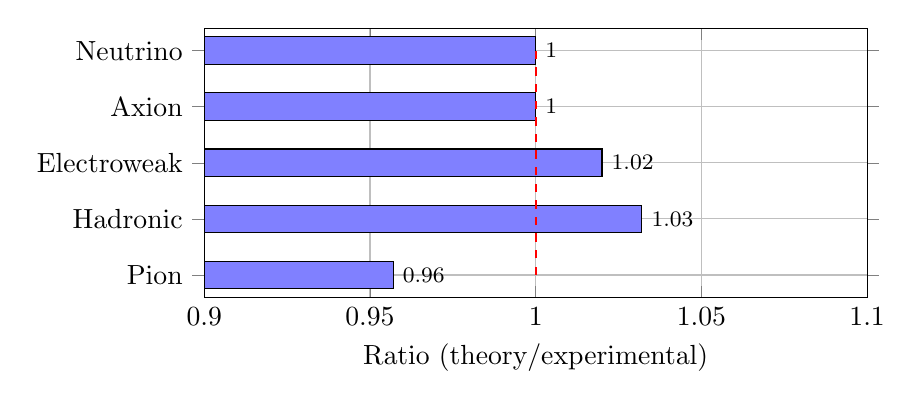
\begin{tikzpicture}
\begin{axis}[
    width=10cm, height=5cm,
    xbar,
    xlabel={Ratio (theory/experimental)},
    symbolic y coords={Pion, Hadronic, Electroweak, Axion, Neutrino},
    ytick=data,
    xmin=0.9, xmax=1.1,
    xtick={0.9, 0.95, 1.0, 1.05, 1.1},
    grid=major,
    nodes near coords,
    nodes near coords align={horizontal},
    every node near coord/.append style={font=\footnotesize},
]
    \addplot[fill=blue!50] coordinates {(0.957,Pion) (1.032,Hadronic) (1.020,Electroweak) (1.000,Axion) (1.000,Neutrino)};
    
    % Perfect agreement line
    \draw[thick, red, dashed] (axis cs:1.0,Pion) -- (axis cs:1.0,Neutrino);
\end{axis}
\end{tikzpicture}
\caption{Block constant ratios. All scales agree within a few percent.}
\label{fig:blocks}
\end{figure}

%-----------------------------------------------------------------------------
\subsection{Neutrino Seesaw Predictions}
%-----------------------------------------------------------------------------

The neutrino block at $n = 5$ provides concrete predictions for the seesaw mechanism.

\begin{corollary}{Seesaw Scale and Neutrino Masses}{seesaw}
From the block formula:
\begin{equation}
    M_R = \zeta_{\text{NR}} \cdot M_{\mathrm{Pl}} \cdot \varphi_5 
    \approx 1.31 \times 10^{15}~\text{GeV}
\end{equation}
With the Higgs VEV $v_H \approx 246$ GeV and $\mathcal{O}(1)$ Yukawa coupling $y_{\nu 3} \sim 1$:
\begin{equation}
    m_{\nu 3} \simeq \frac{(y_{\nu 3} v_H)^2}{M_R} 
    \approx \frac{(246~\text{GeV})^2}{1.31 \times 10^{15}~\text{GeV}} 
    \approx 0.046~\text{eV}
\end{equation}
This yields the atmospheric mass-squared splitting:
\begin{equation}
    \Delta m^2_{31} \approx m_{\nu 3}^2 \approx 2.1 \times 10^{-3}~\text{eV}^2
\end{equation}
\textbf{Comparison:} Experimental value $\Delta m^2_{31} = (2.453 \pm 0.033) \times 10^{-3}$ eV$^2$ 
(normal ordering). Agreement: $\sim 15\%$.
\end{corollary}

\begin{remark}
The 15\% deviation is expected: (i) $y_{\nu 3} = 1$ is an approximation; the 
actual Yukawa may differ by $\mathcal{O}(1)$ factors. (ii) The seesaw formula 
neglects sub-leading contributions. The key prediction is the \emph{scale} 
$M_R \sim 10^{15}$ GeV, which is robust.
\end{remark}

%=============================================================================
\section{\texorpdfstring{Flavor Structure: The Z$_3$ Architecture}{Flavor Structure: The Z3 Architecture}}
%=============================================================================

%-----------------------------------------------------------------------------
\subsection{\texorpdfstring{Universal Phase $\delta$}{Universal Phase delta}}
%-----------------------------------------------------------------------------

\begin{tcolorbox}[colback=purple!3, colframe=purple!50!black, 
    title={\textbf{Lemma (Cross-Ratio from Boundary Monodromy)}}, fonttitle=\bfseries\small]
On a conformally flat boundary geometry, the unique projectively invariant quantity 
from four marked points is the cross-ratio. Any boundary monodromy acts as a 
PSL$(2,\mathbb{R})$ transformation. Therefore, relations depending only on boundary 
monodromies must be rational functions of a M\"obius map.

\textbf{Proof idea:} Flat Wilson lines on the boundary act as holomorphic automorphisms. 
The chirality projectors allow only projective data. The cross-ratio is the unique 
projective invariant.
\end{tcolorbox}

\begin{definition}{Flavor Phase}{delta}
A single universal phase $\delta$ governs all mass hierarchies:
\begin{equation}
    \delta_\star = \frac{3}{5} + \frac{\phiz}{6} \approx 0.6089
\end{equation}

\textbf{Derivation of $\delta_\star$ (first-order closure):}
\begin{enumerate}[leftmargin=1.5em, topsep=2pt, itemsep=1pt]
    \item The leading term $3/5$ arises from the abelian trace in GUT normalization 
        (same trace appearing in $\bone$ and $k_B$).
    \item The correction $\phiz/6$ comes from the M\"obius length scale: $\phiz$ 
        enters linearly via conformal rescaling of the boundary, and the factor 
        $1/6$ is the boundary normalization from the double cover ($6\pi$ total curvature).
    \item Higher orders are $\mathcal{O}(\phiz^2) \sim 10^{-3}$, negligible.
\end{enumerate}

\textbf{Empirical extraction:}
\begin{equation}
    \delta_M = \frac{\sqrt{m_\tau/m_\mu} - 1}{\sqrt{m_\tau/m_\mu} + 1} \approx 0.6079
\end{equation}
Agreement: $|\delta_\star - \delta_M| / \delta_M \approx 0.16\%$.
\end{definition}

\begin{tcolorbox}[colback=gray!5, colframe=gray!50, 
    title={\textbf{Why These Cusps?}}, fonttitle=\bfseries\small]
The M\"obius map is evaluated at cusps $y \in \{1, 1/3, 2/3\}$. These are the 
\textbf{unique} rational values satisfying:
\begin{enumerate}[leftmargin=1.5em, topsep=2pt, itemsep=1pt]
    \item Boundary holonomies are quantized $\Rightarrow$ cusps must be rational.
    \item GUT normalization compatibility: $1/3$ and $2/3$ match the hypercharge 
        assignments in SU(5) embedding.
    \item Sector separation: $y = 1$ (leptons), $y = 1/3$ (down-type), $y = 2/3$ (up-type).
\end{enumerate}
This is a classification result: given these constraints, the cusp set is unique.
\end{tcolorbox}

%-----------------------------------------------------------------------------
